
\documentclass{article}
\usepackage{geometry}
\usepackage{concmath}
\usepackage[OT1]{fontenc}
\usepackage{graphicx}
\usepackage{amsfonts}
\usepackage{amsmath,mathtools}
\usepackage{calrsfs}
\usepackage{color}
\usepackage[dvipsnames]{xcolor}
\usepackage[many]{tcolorbox}
\usepackage{setspace}
\usepackage{tkz-tab}               % for LINE SPACING
\usepackage{multicol}  
\geometry{margin=0.5in}
\definecolor{green}{RGB}{52, 235, 168}
\definecolor{violet}{RGB}{165, 83, 237}
\definecolor{lemon}{RGB}{170, 237, 83}
\definecolor{red}{RGB}{240, 125, 84}
\definecolor{blue}{RGB}{105, 255, 242}


\begin{document}

\noindent \Large
Charlotte WONG\\

\noindent
\colorbox{green}{Exercice 610.20}\\

\large \noindent
On veut étudier la fonction 
\begin{align*}
    f : &\mathbb{R} \rightarrow \mathbb{R}\\
    &x \mapsto Arcsin(\frac{x+1}{\sqrt{2(x^2+1)}})
\end{align*}

\noindent
f est définie sur \(x \in \mathbb{R}\) pour x vérifiant :
\begin{align*}
    &\indent \indent \frac{|x + 1|}{\sqrt{2(x^2+1)}} \leq 1 \text{ car \(\sqrt{2(x^2+1)}\) est toujours positif}\\
    & \Leftrightarrow |x+1| \leq \sqrt{2(x^2+1)}\\
    & \Leftrightarrow (x+1)^2 \leq 2(x^2+1)\\
    & \Leftrightarrow x^2 + 2x + 1 \leq 2(x^2+1)\\
    & \Leftrightarrow 0 \leq 2x^2 - x^2 - 2x -1 + 2\\
    & \Leftrightarrow 0 \leq x^2 - 2x + 1 \\
    & \Leftrightarrow 0 \leq (x-1)^2\\
    & \Leftrightarrow x \in \mathbb{R}
\end{align*}
\noindent
Donc \fbox{f est définie sur \(\mathbb{R}\)}\\

\noindent
\(\frac{x+1}{\sqrt{2(x^2+1)}}\) est continue dans [-1, 1]\\
Donc f est continue par composition de fonctions continues et a pour dérivée 
\begin{align*}
    f'(x) &= \frac{u'(x)}{\sqrt{1-u^2(x)}}\\
    u(x) &= \frac{x+1}{\sqrt{2(x^2+1)}}\\
    u'(x) &= \frac{1\times \sqrt{2(x^2+1)} - (x+1)\times \frac{2x}{\sqrt{2(x^2+1)}}}{2(x^2+1)}\\
    &= \frac{\frac{2(x^2+1)-2x^2-2x}{\sqrt{2(x^2+1)}}}{2(x^2+1)}\\
    &= \frac{\frac{2(1-x)}{\sqrt{2(x^2+1)}}}{2(x^2+1)}\\
    &= \frac{1-x}{\sqrt{2}(x^2+1)^{3/2}}\\
    f'(x) &=  \frac{\frac{1-x}{\sqrt{2}(x^2+1)^{3/2}}}{\sqrt{1-\frac{(x+1)^2}{2(x^2+1)}}}\\
\end{align*}
\begin{align*}
    \Aboxed{f'(x) &= \frac{1-x}{\sqrt{2}(x^2+1)^{3/2}\sqrt{1-\frac{(x+1)^2}{2(x^2+1)}}}}
\end{align*}
\noindent
On a \(\sqrt{1-\frac{(1+1)^2}{2(1^2+1)}} = 0\) donc \underline{f' n'est pas définie en 1}\\
On a aussi pour x non nul: 
\begin{align*}
    f(x) &= Arcsin(\frac{x(1+1/x)}{\sqrt{2x^2(1+1/x^2)}})\\
    &= Arcsin(\frac{x}{|x|} \frac{1+1/x}{\sqrt{2(1+1/x^2)}})\\
    &= \begin{cases*}
        Arcsin(-\frac{1+1/x}{\sqrt{2(1+1/x^2)}}), \text{ si }x < 0\\
        Arcsin(\frac{1+1/x}{\sqrt{2(1+1/x^2)}}), \text{ si } x > 0
    \end{cases*}
\end{align*}
Donc \begin{align*}
    &\frac{1+1/x}{\sqrt{2(1+1/x^2)}} \to_{x\to +\infty} \frac{1}{\sqrt{2}}\\
    \Leftrightarrow &f(x) \to_{x\to +\infty} \frac{\pi}{4}\\
    &-\frac{1+1/x}{\sqrt{2(1+1/x^2)}} \to_{x\to -\infty} -\frac{1}{\sqrt{2}}\\
    \Leftrightarrow &f(x) \to_{x\to -\infty} -\frac{\pi}{4}
\end{align*}
\noindent
f' est du signe de 1-x et donc on obtient le tableau de variation suivant :\\

\normalsize
\begin{tikzpicture}
\tkzTabInit[espcl=3,lgt=2]
  {$x$/1, $f'(x)$/1, $f(x)$/2}
  {$-\infty$, 1, $+\infty$}
\tkzTabLine{ , +, ||, -, }
\tkzTabVar{
  -/$-\dfrac{\pi}{4}$/,
  +/$\dfrac{\pi}{2}$/,
  -/$\dfrac{\pi}{4}$/
}
\end{tikzpicture}\\

\large
\noindent
Et l'allure de la courbe de f est : \\
\noindent
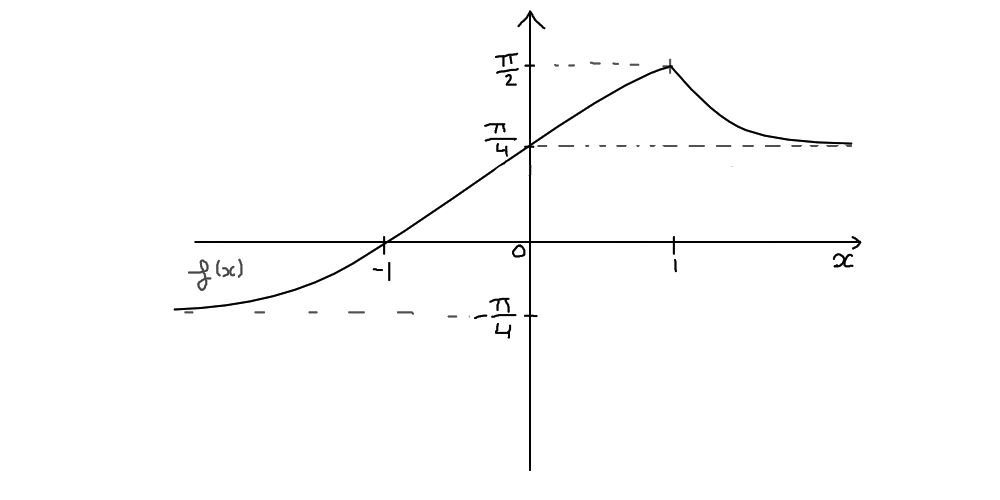
\includegraphics[scale = 3.6]{fonction-61020.jpg}


\Large \noindent
\colorbox{green}{Ex 610.21}\\
\large \noindent
a/ \begin{align*}
    &\frac{1}{p^2+p+1} = \frac{1}{p^2}\frac{1}{1+1/p+1/p^2}\\
\end{align*} 
quand \(p \to +\infty\)
\begin{align*}  
    &\frac{1}{1+1/p+1/p^2} = 1 + o(1)\\
\end{align*}
Donc \begin{equation*}
    \frac{1}{p^2+p+1} = \frac{1}{p^2}(1+o(1))
\end{equation*}
Donc \begin{equation*}
    \frac{1}{p^2+p+1} \sim \frac{1}{p^2} \text{ quand \(p \to +\infty\)}
\end{equation*}
Donc \begin{align*}
    Arctan(\frac{1}{p^2+p+1}) &\sim \frac{1}{p^2+p+1}\\
    &\sim \frac{1}{p^2}
\end{align*}
Or la série de terme général \(\frac{1}{p^2}\) converge\\
Donc \fbox{la série de terme général \(u_p\) converge}\\
\noindent
b/ \begin{align*}
    tan(Arctan(p+1)-Arctan(p)) &= \frac{p+1-p}{1+(p+1)p}\\
    &= \frac{1}{p^2+p+1}\\
    \Aboxed{Arctan(p+1)-Arctan(p) &= Arctan(\frac{1}{p^2+p+1})}
\end{align*}
\noindent
c/ D'après b/\\
\begin{align*}
    \sum_{p=0}^{+\infty} u_p = \sum_{p=0}^{+\infty} Arctan(p+1)-Arctan(p)
\end{align*}
Par télescopage et en passant par la limite
\begin{align*}
    &Arctan(p) \to_{p\to +\infty} \frac{\pi}{2}\\
    \Aboxed{&\sum_{p=0}^{+\infty} u_p = \frac{\pi}{2}}
\end{align*}


\end{document}